



 $\Delta ABC$ and $\Delta GHI$ are equilateral triangles with perimeter 9 and triangle $\Delta DEF$ is an equilateral triangle with perimeter 12.  If $AI = 8$ and $ DC=GF$, then what is the perimeter of the bolded region?
 \begin{center}
 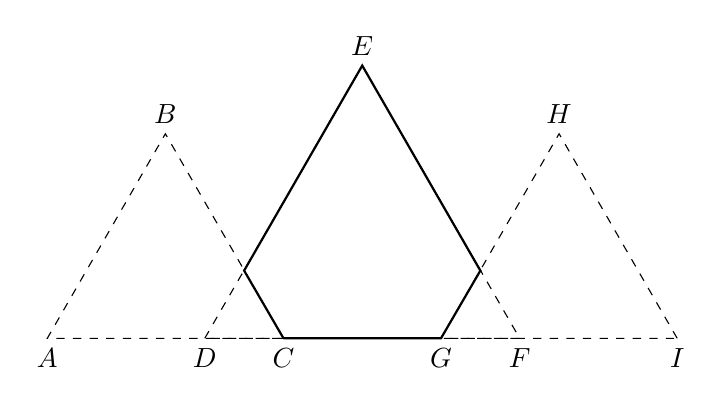
\begin{tikzpicture}
 
  
  
    \draw (0,0) -- (2,.866*4)--(4,0)--(0,0)[thin, dashed,-,>=latex];
  
  \draw (1,0) -- (-.5,.866*3)--(-2,0)--(1,0)[thin, dashed,-,>=latex];
  \draw (1+5,0) -- (-.5+5,.866*3)--(-2+5,0)--(6,0)[thin, dashed,-,>=latex];
  
  \draw (1,0)--(.5,.86)--(2,.866*4)--(3.5,.86)--(3,0)--(1,0)[thick,-,>=latex];
  \draw node[below] at (0,0) {$D$};    
  \draw node[below] at (-2,0) {$A$};
   \draw node[below] at (6,0) {$I$};
   \draw node[above] at (2,.866*4) {$E$};
   \draw node[below] at (4,0) {$F$};
   \draw node[below] at (3,0) {$G$};
     \draw node[below] at (1,0) {$C$};
     \draw node[above] at (-.5,.866*3) {$B$};
     \draw node[above] at (-.5+5,.866*3) {$H$};
                                        
      
  
\end{tikzpicture}
\end{center}



\ifsat
	\begin{enumerate}[label=\Alph*)]
		\item  $8$
		\item  $9$  
		\item  $10$ %
		\item  $12$
	\end{enumerate}
\else
\fi

\ifacteven
	\begin{enumerate}[label=\textbf{\Alph*.},itemsep=\fill,align=left]
		\setcounter{enumii}{5}
		\item  $8$
		\item  $9$  
		\item  $10$ %
		\addtocounter{enumii}{1}
		\item  $11$
		\item  $12$
	\end{enumerate}
\else
\fi

\ifactodd
	\begin{enumerate}[label=\textbf{\Alph*.},itemsep=\fill,align=left]
		\item  $8$
		\item  $9$  
		\item  $10$ %
		\item  $11$
		\item  $12$
	\end{enumerate}
\else
\fi

\ifgridin
  $10$ %
		
\else
\fi

